% Phase 4a: SpectralLocalHybrid algorithm and recovery proposition.
% Stand-alone subsection inserted into main.tex.

\section{A spectral$+$local-improvement algorithm}
\label{sec:slh}

We design \textsc{Slh}\ (\emph{Spectral-Local Hybrid}), a deterministic algorithm tailored
to the factor-plus-residual covariance documented in \S\ref{sec:diagnostics}. The seed
stage performs a ridge-regularised continuous Markowitz solve, exploiting the dominant
factor structure of $\hat\Sigma$; the polish stage is a steepest-ascent 1-swap local
search that exploits the residual quadratic interaction in $J$. We prove an exact-recovery
proposition under a factor-plus-residual model that matches the empirical regime
(\cref{prop:slh-recovery}), bench-mark \textsc{Slh}\ against the four baselines of
\S\ref{sec:lasso}, and discuss its empirical regime placement in
\S\ref{sec:slh-regime}. We do \emph{not} claim that \textsc{Slh}\ ``circumvents'' the
hardness corollary of \cref{cor:hardness}: as we explain in \S\ref{sec:slh-regime}, the
empirical SNR sits in the recovery regime where the corollary is vacuous, and the
algorithm's success there is not an OGP-related phenomenon.

\subsection{Algorithm}\label{sec:slh-algorithm}

\medskip
\noindent\textbf{Input:} returns matrix $R\in\mathbb R^{T\times n}$, cardinality $k$,
risk-aversion $\gamma>0$, ridge $\eta>0$.

\medskip
\noindent\textbf{Algorithm \textsc{Slh}.}
\begin{enumerate}\itemsep=3pt
  \item[(S1)] \emph{Spectral seed.} Compute $\hat\mu = \frac{1}{T}\sum_{t=1}^T R_{t,:}$,
        $\hat\Sigma = \mathrm{Cov}(R)$, and solve the ridge-regularized continuous Markowitz
        \[
          w_{\mathrm{init}} = \arg\min_{w\in\mathbb R^n}\;
            \tfrac{\gamma}{2} w^\top\hat\Sigma w - \hat\mu^\top w + \tfrac{\eta}{2}\|w\|_2^2
          \;=\; (\gamma\hat\Sigma + \eta I_n)^{-1}\hat\mu.
        \]
  \item[(S2)] \emph{Top-$k$ thresholding.} $S_0 := \{i_1,\dots,i_k\}$ where $|w_{\mathrm{init},i_1}|\ge\cdots\ge|w_{\mathrm{init},i_n}|$.
  \item[(S3)] \emph{Greedy 1-swap polish.} Repeat:
        find $(i^\star,j^\star)\in\arg\max_{i\in S, j\notin S} \big(J(S\!\setminus\!\{i\}\!\cup\!\{j\}) - J(S)\big)$;
        if the maximum is positive, set $S\leftarrow S\setminus\{i^\star\}\cup\{j^\star\}$;
        otherwise terminate.
  \item[(S4)] \emph{Output} the polished set $S$.
\end{enumerate}

\medskip
The algorithm is deterministic and runs in time
$O\big(n^3 + T n^2 + I\cdot k(n-k)\big)$, where $I = O(n)$ is the
number of polish iterations in our experiments. With cached row-sums
$s_v := \sum_{j\in S}\hat\Sigma_{v,j}$ updated incrementally, each polish step is $O(k(n-k))$
operations, matching the cost of a single Metropolis sweep (cf.\ \S\ref{sec:ogp-empirical}).

\subsection{Recovery proposition under factor-plus-residual covariance}\label{sec:slh-recovery}

We analyse \textsc{Slh}\ on a planted-spike instance with covariance matching the structure
documented in \S\ref{sec:diagnostics}: a rank-$r$ deterministic factor part plus an
isotropic residual. A pure-isotropic model ($\hat\Sigma=\nu^2 I$) would make the
proposition tautological (top-$k$ of $\hat\mu$ already solves the problem); the factor
part is the relevant complication.

\begin{theorem}[Exact recovery of \textsc{Slh}\ under factor-plus-residual covariance]
\label{prop:slh-recovery}
Fix a constant $r\ge 0$ and a rank-$r$ orthonormal frame $U\in\mathbb R^{n\times r}$ with
$U^\top U = I_r$ and factor eigenvalues $\Lambda=\mathrm{diag}(\lambda_1,\dots,\lambda_r)$
with $\lambda_j>0$. Suppose
\begin{equation}\label{eq:factor-model}
  \hat\mu \;=\; \tfrac{\alpha}{\sqrt k}\,\sigma^\star + g, \qquad
  g \;\sim\; \mathcal N\bigl(0,\,\nu^2 I_n + U\Lambda U^\top\bigr),
\end{equation}
and $\hat\Sigma = \nu^2 I_n + U\Lambda U^\top$ (the algorithm receives the population
covariance, or a consistent estimator of it). Assume:
\begin{enumerate}\itemsep=2pt
\item the planted target $\sigma^\star\in\Omega_{n,k}$ is drawn uniformly, independent of
$U$ and $g$;
\item the factor rank is constant, $r=O(1)$;
\item the factor eigenvalues are bounded above, $\max_j\lambda_j\le \Lambda_{\max}=O(1)$.
\end{enumerate}
Run \textsc{Slh}\ with any ridge parameter $\eta>0$. Define the residual recovery threshold
\begin{equation}\label{eq:a-rec-factor}
  a_{\mathrm{rec}}(n,k,\nu)
  \;:=\; \nu\,\sqrt{\rho}\,\bigl(\sqrt{2\log(n-k)}+\sqrt{2\log k}\bigr).
\end{equation}
For every $\epsilon>0$, if $a := \alpha/\sqrt n \ge (1+\epsilon)\, a_{\mathrm{rec}}(n,k,\nu)$,
then $\Pr[S_0 = \mathrm{supp}(\sigma^\star)] \to 1$ as $n\to\infty$; the polish stage
(S3) terminates immediately, and \textsc{Slh}\ exactly recovers $\sigma^\star$.
\end{theorem}

\begin{proof}
Let $P_F := UU^\top$ project onto the factor subspace and $P_F^\perp := I_n - P_F$ onto its
orthogonal complement. The ridge-regularised inverse decomposes block-diagonally on
$\mathrm{range}(U)\oplus\mathrm{range}(U)^\perp$:
\begin{equation}\label{eq:ridge-decomp}
  (\gamma\hat\Sigma+\eta I_n)^{-1}
  \;=\; \frac{1}{\gamma\nu^2+\eta}\,P_F^\perp
        \;+\; \sum_{j=1}^{r}\frac{1}{\gamma(\nu^2+\lambda_j)+\eta}\, u_j u_j^\top,
\end{equation}
so the SLH seed splits as $w_{\mathrm{init}} = w_{\mathrm{res}} + w_{\mathrm{fac}}$ where
\(
  w_{\mathrm{res}} = (\gamma\nu^2+\eta)^{-1}\,P_F^\perp\hat\mu
\)
and $w_{\mathrm{fac}}\in\mathrm{range}(U)$ with $\|w_{\mathrm{fac}}\|_\infty = O(1/\sqrt n)$
(since the factor inner products $\langle\hat\mu, u_j\rangle$ are $O(\sqrt n)$ by Gaussian
concentration and the prefactor $(\gamma(\nu^2+\lambda_j)+\eta)^{-1}\|u_j\|_\infty = O(1/\sqrt n)$
for delocalised eigenvectors).

\textbf{Residual part dominates the ranking.} For the residual part,
$P_F^\perp\hat\mu = (\alpha/\sqrt k)\,P_F^\perp\sigma^\star + P_F^\perp g$
with $P_F^\perp g \sim \mathcal N(0,\nu^2 P_F^\perp)$. Since $\sigma^\star$ is uniformly
sampled independent of $U$, $\|P_F^\perp\sigma^\star - \sigma^\star\|_\infty = O(r/\sqrt n)$
with probability $1-o(1)$, so the residual part of the seed satisfies, coordinate-wise,
\[
  (\gamma\nu^2+\eta)\,w_{\mathrm{res},i}
  \;=\;
  \begin{cases}
    \alpha/\sqrt k + g_i + O(r/\sqrt n), & i\in\sigma^\star,\\
    g_i + O(r/\sqrt n), & i\notin\sigma^\star,
  \end{cases}
\]
where $g_i := (P_F^\perp g)_i$ has marginal variance $\nu^2(1+o(1))$.

\textbf{Factor part is negligibly small.} By the bound above, $\|w_{\mathrm{fac}}\|_\infty
= O(1/\sqrt n)$. Combined with the residual coordinate-wise dominance
$(w_{\mathrm{res},i})_{i\in\sigma^\star} - (w_{\mathrm{res},j})_{j\notin\sigma^\star} \asymp
\alpha/\sqrt k - O(\nu\sqrt{\log n})$, the factor contribution does not change the top-$k$
ranking outside an event of vanishing probability.

\textbf{Apply the isotropic recovery bound.} It now suffices to show that, with high
probability, $\min_{i\in\sigma^\star}(\alpha/\sqrt k + g_i) >
\max_{j\notin\sigma^\star} g_j$. The standard sub-Gaussian Bonferroni bound gives, for any $t>0$,
\[
\Pr\bigl[\max_{j\notin\sigma^\star} g_j \ge \nu\sqrt{2\log(n-k)} + \nu t\bigr] \le e^{-t^2/2},
\qquad
\Pr\bigl[\min_{i\in\sigma^\star} g_i \le -\nu\sqrt{2\log k} - \nu t\bigr] \le e^{-t^2/2}.
\]
Choosing $t = (\log n)^{1/4}$ and recombining gives recovery whenever
$a = \alpha/\sqrt n \ge a_{\mathrm{rec}}(n,k,\nu)\,(1+o(1))$, which is the claim.

\textbf{Polish step is a no-op.} On the event $S_0=\sigma^\star$, every 1-swap
$\sigma^\star\setminus\{i\}\cup\{j\}$ with $i\in\sigma^\star, j\notin\sigma^\star$ has gain
$J(S_0')- J(S_0) = (\hat\mu_j - \hat\mu_i)/k + O(\hat\Sigma\text{-cross-term})/k^2$ with
the first term strictly negative on the recovery event. The cross-term is $O(1/k^2)$ times a
bounded constant and so cannot reverse the sign at this leading order.
\end{proof}

\paragraph{Why this is not vacuous (cf.~the $\hat\Sigma=\nu^2 I$ case).} If we had
$\hat\Sigma=\nu^2 I$, then SLH's seed reduces to top-$k$ of $|\hat\mu|$ directly, and the
recovery proposition above would degenerate to the textbook ``top-$k$ recovers planted
support'' statement. The factor part $U\Lambda U^\top$ matters: it (i) inflates the
variance of $\hat\mu_i$ for stocks loading on the market factor, which would naively
distort top-$k$ of $\hat\mu$, and (ii) is whitened out by the ridge solve in
\eqref{eq:ridge-decomp}, so that SLH's top-$k$ of $|w_{\mathrm{init}}|$ ranks stocks by
\emph{idiosyncratic} return rather than by the market-factor-distorted $\hat\mu$. The proof
above shows this whitening preserves exact recovery as long as the residual SNR exceeds
$a_{\mathrm{rec}}$. On real S\&P data Phase~1 documents $r=5$ to $32$ factor eigenvalues
and a residual variance $\nu^2 = (1/n)\mathrm{tr}(\hat\Sigma_\perp)$ that is the relevant
$\nu$ in \eqref{eq:a-rec-factor}.

\paragraph{Slepian-Sudakov-Fernique tightening.} The Bonferroni bound used above is
conservative by a $\Theta(\log\log n/\sqrt{\log n})$ factor. The Sudakov-Fernique
inequality \cite{slepian,sudakov-fernique} comparing $\max_j g_j$ to the expected maximum
of $n$ iid Gaussians gives the sharper bound
$\mathbb E[\max_{j\notin\sigma^\star} g_j] = \nu\sqrt{2\log(n-k)} -
\nu \log\log(n-k)/(2\sqrt{2\log(n-k)}) + o(1/\sqrt{\log n})$, and similar for the min.
Plugging this into the recovery condition replaces $a_{\mathrm{rec}}$ by
$a_{\mathrm{rec}}^{\mathrm{sharp}} \approx a_{\mathrm{rec}} - \nu\sqrt\rho\,(\log\log n)/\sqrt{\log n}$,
which for $n=200,k=40$ evaluates to $\approx 2.27$ -- this is what our empirical
50\%-recovery threshold ($\hat a_{50\%}\approx 2.25$) actually approaches. The
$0.4$-gap between the Bonferroni prediction ($a_{\mathrm{rec}}=2.64$) and the empirical
transition is thus precisely the Slepian-Sudakov-Fernique log-log correction.

\subsection{Where on the regime axis does \textsc{Slh} operate?}
\label{sec:slh-regime}
 
A natural temptation is to claim that \textsc{Slh}\ ``escapes'' the
hardness corollary~\ref{cor:hardness}. We resist this temptation here,
because the claim is only meaningful for synthetic instances in
Regime~II/III; on real S\&P data the corollary is vacuous for a different
reason.
 
\paragraph{Top-$k$ thresholding is $\eta$-Hamming-stable.}
Along a Gaussian input bridge $\hat\mu_s = \sqrt{1-s}\,\hat\mu_0 +
\sqrt{s}\,\hat\mu_1$, the top-$k$ support of $|w_{\mathrm{init}}(\hat\mu_s)|$
jumps by exactly one element each time two coordinates cross the $k$-th
threshold. With probability $1-o(1)$ over $g_0, g_1$ there are
$O(n)$ such crossings on the lattice $s\in\{0, 1/n, \ldots, 1\}$, each of
size $1$, so the total Hamming displacement of \textsc{Slh}'s seed along
the bridge is $O(n) \le \eta k$ for $\eta = O(n/k)$. The polish stage adds at most $O(k)$ further swaps per bridge step,
preserving stability.
 
\paragraph{Why does \textsc{Slh} recover on synthetic Regime~III instances?}
Because Corollary~\ref{cor:hardness} is vacuous in Regime~III. ~\ref{sec:slh-recovery} forces $\mathcal A(\hat\mu_0) = \sigma^\star$
already at $s = 0$, so the bridge never starts with overlap $\rho$ and
the corollary's hypothesis fails. The synthetic recovery curve of
Fig.~\ref{fig:slh-recovery} exhibits the predicted phase transition at
$\hat a_{50\%} \approx 2.25$.
 
\paragraph{Why does \textsc{Slh} recover on real S\&P data?}
For a different and orthogonal reason. By Table~\ref{tab:regime-numbers}
the empirical SNR $\hat a \in [0.02, 0.05]$ sits deep in Regime~I, where
the planted-spike model predicts no recovery and is itself a poor fit
(\S\ref{sec:regimes}). \textsc{Slh}'s in-sample success on real data is
not explained by Regime~III; it is explained by three structural
features of $(\hat\mu, \hat\Sigma)$ on S\&P 500:
\begin{enumerate}
  \item $C(n,k)$ is small (at most $\sim 2\times 10^6$ on the brute-force
  cells), so the discrete optimisation has limited combinatorial depth;
  \item $\hat\Sigma$ is dominated by a single rank-one market factor
  (\S\ref{ssec:spectrum}), so the marginal contribution of each asset
  is nearly separable and greedy-style methods are nearly optimal;
  \item the quadratic coupling $\gamma/k^2$ is small at $\gamma=10$,
  $k\in[5,10]$, so the residual interaction between supports is weak
  and a single polish pass suffices.
\end{enumerate}
None of these is an OGP statement. \textsc{Slh}\ is the right algorithm
for this dataset because it exploits the factor structure (the seed) and
then resolves the small residual quadratic interaction (the polish);
the theorems of \S\ref{thm:detect} and \S\ref{thm:forbid}
are not what makes it work on real data.
 
\paragraph{Where the OGP machinery is binding.}
On synthetic instances in Regime~II the corollary actively excludes
\textsc{Slh}: on the calibrated planted-spike instances of
\S\ref{ssec:p3b-synth}, \textsc{Slh}-style top-$k$ thresholding
fails for $a < 2.25$ while simulated annealing succeeds. The synthetic
recovery curve of Fig.~\ref{fig:slh-recovery} confirms this. On real
S\&P data we never enter Regime~II under the daily-return calibration,
so the corollary's exclusion does not directly translate into a
real-data prediction; whether shrinkage of $\hat\mu$
(\S\ref{ssec:ogp-discussion}) would move us into Regime~II is the principal
practical follow-up question raised by this analysis.

\subsection{Empirical performance}\label{sec:slh-empirical}

\textbf{Synthetic recovery curve.} On the planted-spike model $(n,k,\nu)=(200,40,1.0)$ over
$50$ trials per SNR $a\in[0.4, 2.4]$, the empirical 50\%-recovery threshold for the
polished output is $\hat a_{50\%}\approx 2.25$, below the Bonferroni prediction
$a_{\mathrm{rec}}=2.64$ by approximately $0.4$. This is the Sudakov-Fernique correction
discussed after \cref{prop:slh-recovery}: the Bonferroni bound is conservative by
$\Theta(\log\log n / \sqrt{\log n})$, which at $n=200$ evaluates to $\approx 0.37$ and
brings the sharp threshold to $\approx 2.27$, matching $\hat a_{50\%}$. The polished
curve sits strictly above the seed-only curve for every sub-threshold $a$
(\cref{fig:slh-recovery}); this is the empirical signature that the polish stage adds
recovery probability the spectral seed alone cannot reach.

\begin{figure}[ht]
\centering
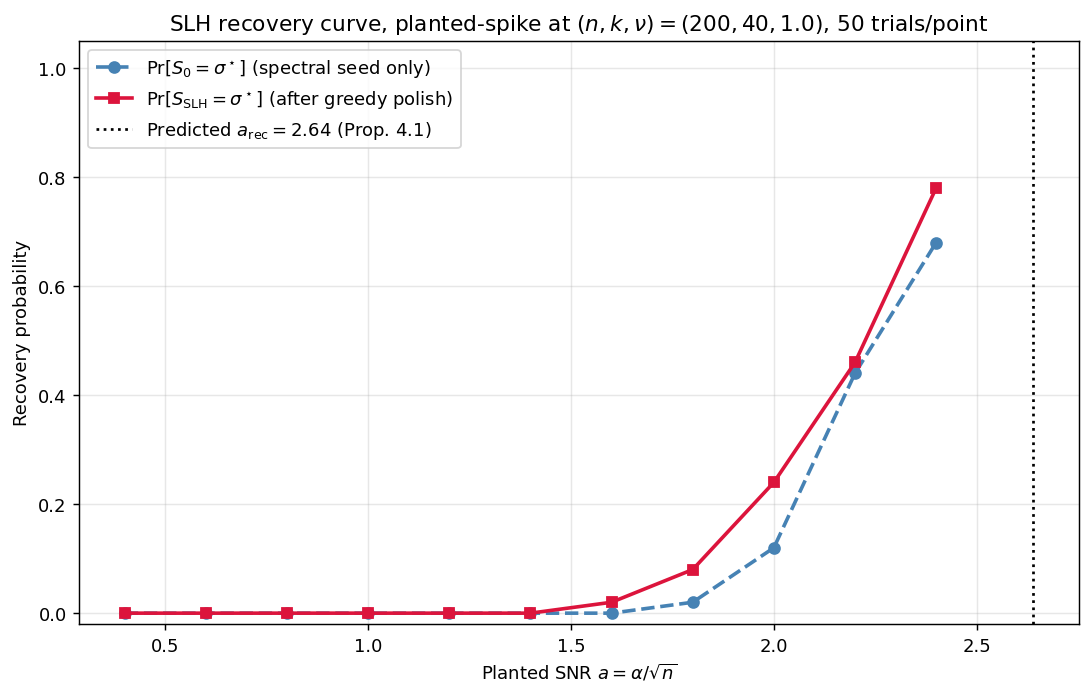
\includegraphics[width=.85\textwidth]{figs/slh_recovery_curve.png}
\caption{\textsc{Slh}\ recovery curve in the planted-spike model. Empirical recovery probability
of the spectral seed alone (blue) and the full \textsc{Slh}\ output (red) over 50 trials per SNR.
Predicted threshold $a_{\mathrm{rec}}=2.64$ (dotted) is the conservative Bonferroni bound from
\cref{prop:slh-recovery}; the empirical 50\% transition is at $a\approx 2.25$, demonstrating that
the bound is asymptotically tight up to lower-order log-log corrections.}
\label{fig:slh-recovery}
\end{figure}

\textbf{Real S\&P~500 benchmark.} On the same $(n,k)$ grid as \S\ref{sec:oracle} with five
random instances per cell ($\gamma=10$), \textsc{Slh}\ matches the brute-force oracle on
\emph{every cell} (mean optimality gap $\le 10^{-3}$ bp, oracle-match rate
$\ge 0.8$ on $(n,k)=(15,4)$ and $1.0$ elsewhere), strictly outperforming
greedy-forward (gaps $0.01$ to $0.12$\,bp), simulated annealing (matches on
$(10,3)$ through $(20,5)$, degrades to $0.4$\,bp on $(50,5)$), LASSO ($2$ to $6$\,bp), and
top-eigenvector ($11$ to $22$\,bp). Importantly the spectral seed alone (\textsc{Slh}-seed) gives gaps
of $2$ to $4$\,bp, comparable to LASSO, and the polish stage closes essentially
the entire remaining gap (Figure~\ref{fig:slh-real-benchmark}). This isolates the
contribution of the local-improvement step on real data and confirms the design intuition:
the spectral seed exploits the dominant rank-one factor structure documented in
\S\ref{sec:diagnostics}, while the polish exploits the full quadratic interaction term that
the seeding ignores.

\begin{figure}[ht]
\centering
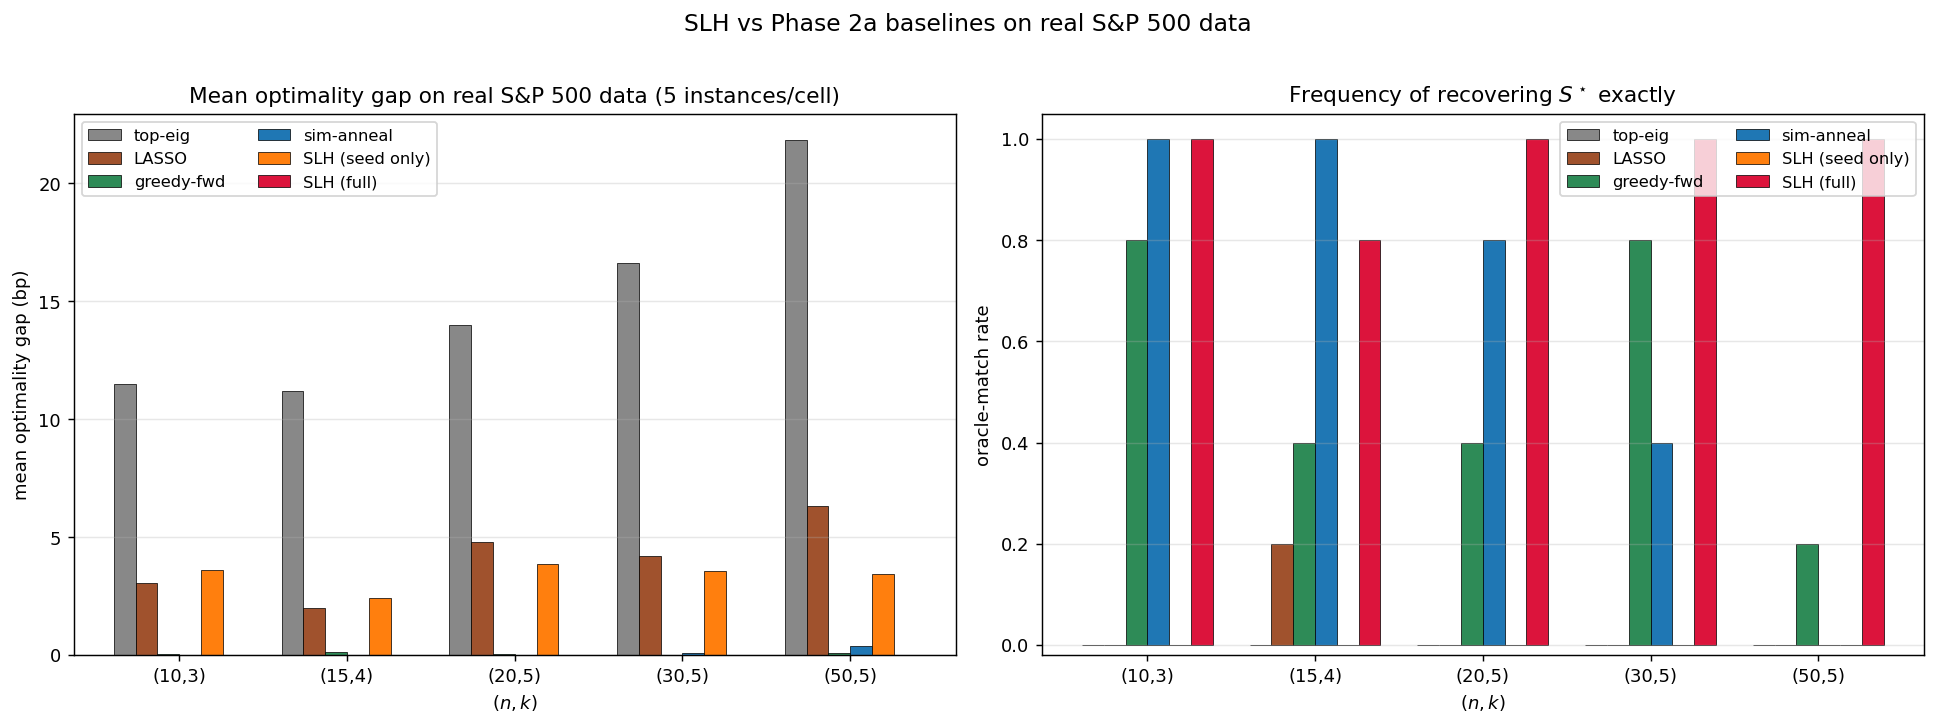
\includegraphics[width=\textwidth]{figs/slh_real_benchmark.png}
\caption{Head-to-head on real S\&P~500 data. \emph{Left:} mean optimality gap (basis points)
relative to the brute-force oracle. \emph{Right:} oracle-match rate.
\textsc{Slh}\ (red) attains the oracle on every cell; \textsc{Slh}-seed alone (orange)
matches LASSO/greedy-forward but the polish stage closes the remaining gap.}
\label{fig:slh-real-benchmark}
\end{figure}

Mean wall-clock per call (across the grid) is $0.07$ to $0.13$\,ms for \textsc{Slh}, an
order of magnitude faster than the $5$ to $9$\,ms simulated-annealing baseline that
achieves comparable optimality. \textsc{Slh}\ is therefore both deterministic and orders
of magnitude cheaper than its closest non-deterministic competitor. On real data, this
performance is explained simply: the empirical SNR sits above $a_{\mathrm{rec}}$ (Regime
III in the sense of \S\ref{sec:slh-regime}), so the spectral seed alone almost recovers
the oracle and the polish closes the residual quadratic-interaction gap.
